\chapter{Analysis and Results}\label{chapter:Results}

\section{Findings with Respect to Hypothesis}

\subsection{Ajzen Model}

\subsubsection{Regression Outcome}
\begin{table}[H]
\centering
\caption{Residuals}
\label{Residuals}
\begin{tabular}{@{}lllll@{}}
\toprule
Min      & 1Q       & Median  & 3Q      & Max     \\ \midrule
-1.50912 & -0.49199 & 0.05257 & 0.40802 & 1.51899 \\ \bottomrule
\end{tabular}
\end{table}

\begin{table}[H]
\centering
\caption{Coefficients}
\label{Coefficients}
\begin{tabular}{@{}llllll@{}}
\toprule
            & Estimate & Std. Error & t value & Pr(\textgreater|t|) & Signif. code \\ \midrule
(Intercept) & -2.16529 & 1.22500    & -1.768  & 0.08205             & .            \\
PA          & 0.77889  & 0.07090    & 10.985  & 3.49e-16            & ***          \\
SN          & 0.24256  & 0.20387    & 1.190   & 0.23867             &              \\
PBC         & 0.24723  & 0.08495    & 2.910   & 0.00501             & **           \\ \bottomrule
\end{tabular}
\end{table}

Signif. codes:  0 '***' 0.001 '**' 0.01 '*' 0.05 '.' 0.1 ' ' 1

Residual standard error: 0.7357 on 62 degrees of freedom
Multiple R-squared:  0.8182,	Adjusted R-squared:  0.8094 
F-statistic: 93.01 on 3 and 62 DF,  p-value: < 2.2e-16


\subsubsection{Plotted Variables}

\begin{figure}[H]
\centering{
\caption{EI vs PA}
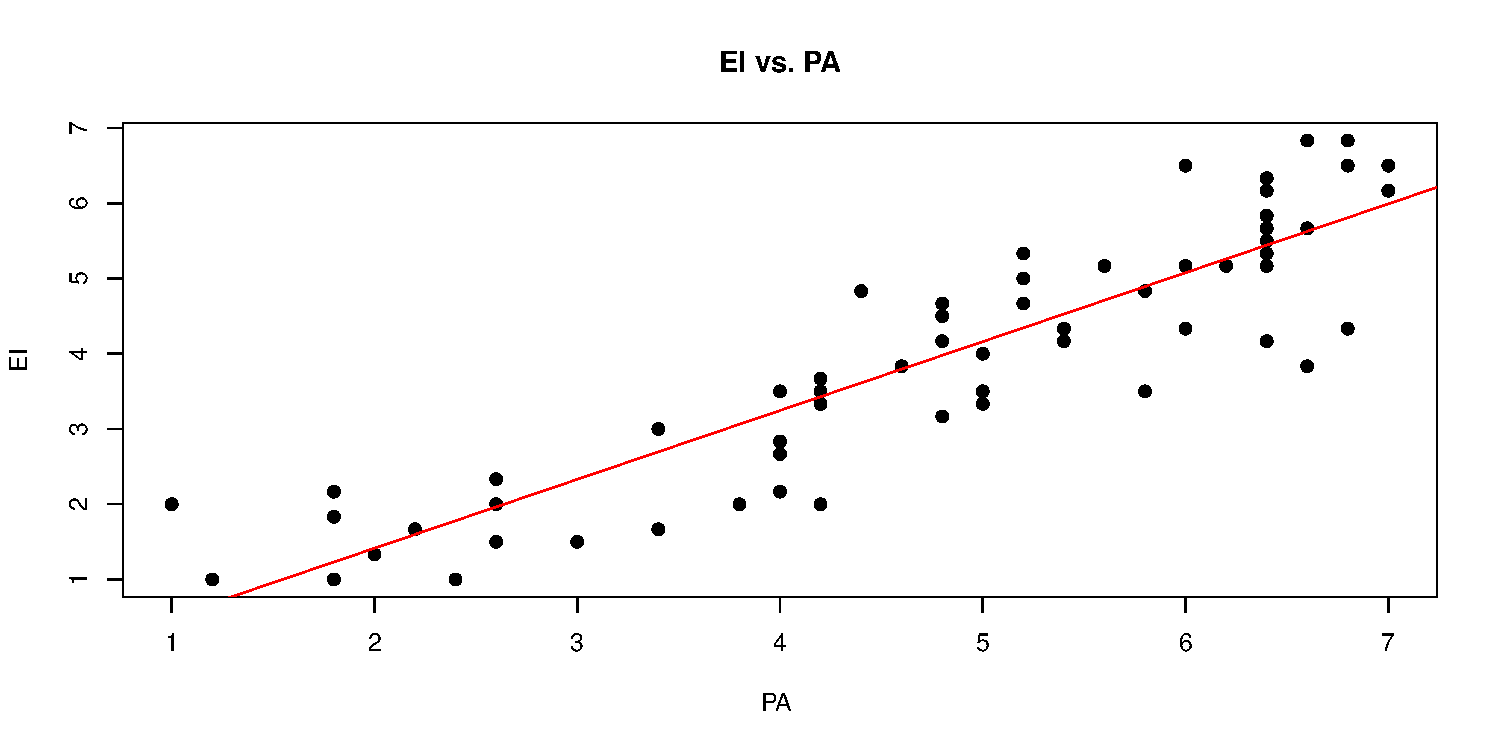
\includegraphics[width=\textwidth,keepaspectratio]{images/EIvsPA.pdf}}
\end{figure}

\begin{figure}[H]
\centering{
\caption{EI vs SN}
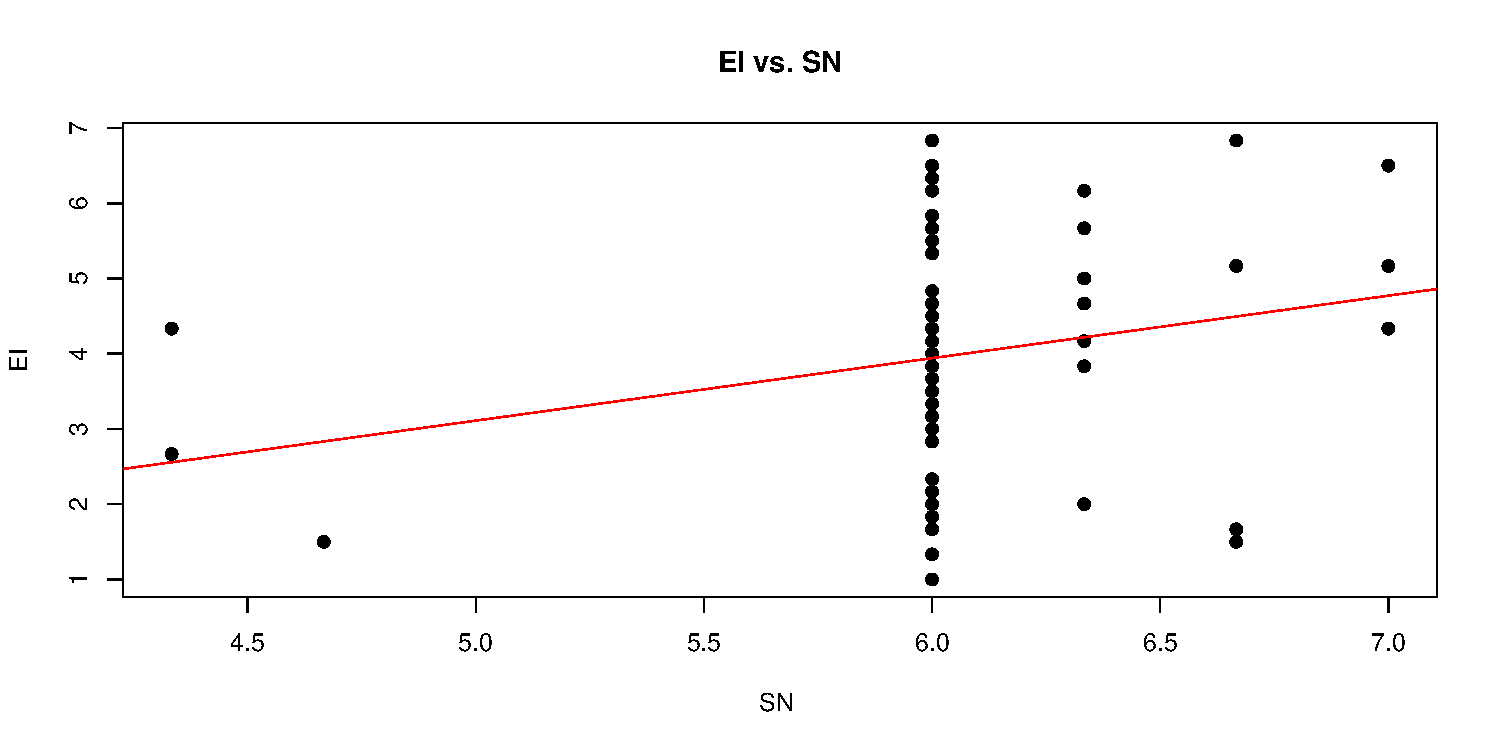
\includegraphics[width=\textwidth,keepaspectratio]{images/EIvsSN.pdf}}
\end{figure}

\begin{figure}[H]
\centering{
\caption{EI vs PBC}
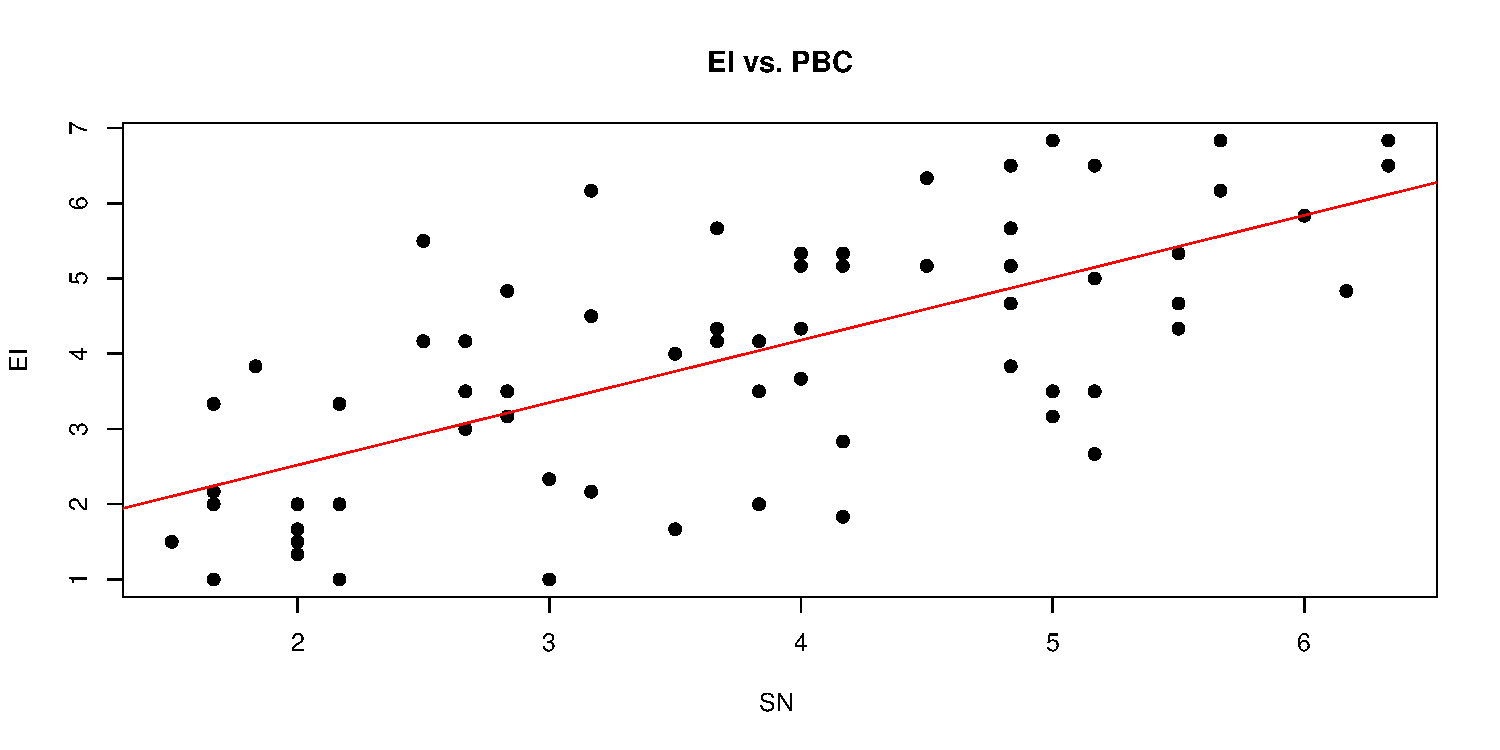
\includegraphics[width=\textwidth,keepaspectratio]{images/EIvsPBC.pdf}}
\end{figure}

